\chapter{Программная реализация}

\section{Веб-интерфейс}
Веб-интерфейс является важнейшим элементом пользовательского взаимодействия с системой, обеспечивая доступ ко всему спектру функциональных возможностей приложения Bishop.
В данной главе будет рассмотрена структура интерфейса, описаны отдельные страницы и реализуемые ими задачи, а также представлен детальный анализ технических решений,
используемых при разработке.

\subsection{Гостевая страница}
Первая страница веб-интерфейса, доступная пользователю, представляет собой гостевую посадочную страницу \ref{fig:ui-page-welcome} (landing page). Она разработана с целью ознакомления пользователей с проектом Bishop и не требует предварительной авторизации.


Страница выполнена в минималистичном стиле, что позволяет сфокусировать внимание пользователя на основном содержании. В верхней части расположено название проекта «Bishop Ai Application», а справа в шапке страницы находятся две активные ссылки: «Login» и «Signup», позволяющие перейти к авторизации или регистрации соответственно.


Центральная часть страницы содержит краткое приветствие пользователя («Welcome to BishopApp») и детальное описание основной идеи и функционала приложения. 


Нижний колонтитул страницы содержит информацию об авторских правах, что завершает композицию интерфейса и подчеркивает официальность ресурса.

\subsection{Идентификация, аутентификация и авторизация}

Сервис Bishop предусматривает возможность идентификации и авторизации пользователей через формы 
входа \ref{fig:ui-page-login} («Login») и регистрации \ref{fig:ui-page-signup} («Signup»).

Страница входа содержит поля для ввода электронной почты и пароля. После отправки данных 
производится запрос к backend API, который проверяет подлинность введенных данных. В случае 
успешного входа система переадресует пользователя на личную страницу, при этом отображая 
уведомление с текстом «login is successful!». Если данные введены неверно, интерфейс 
отображает сообщение об ошибке («Incorrect email or password»), что существенно улучшает 
пользовательский опыт, четко информируя о причинах невозможности авторизации.

\subsubsection{Регистрация}

Форма регистрации аналогична форме входа, однако требует от пользователя дополнительной информации 
в виде полного имени. Введенные данные валидируются как на уровне фронтенда (проверка 
формата email и минимальной длины пароля), так и на стороне бэкенда (проверка уникальности email). 
Ошибки ввода или проверки также сопровождаются информативными уведомлениями:

\begin{itemize}
  \item \texttt{value is not a valid email address} — если указан некорректный адрес электронной почты.
  \item \texttt{String should have at least 8 characters} — при слишком коротком пароле.
  \item \texttt{The user with this email already exists in the system} — если email уже зарегистрирован.
\end{itemize}

\subsubsection{Техническая реализация и безопасность данных}

Для реализации процесса авторизации используется стандарт JWT. После успешной 
аутентификации токен сохраняется в сессии пользователя и добавляется в заголовки каждого запроса 
к backend API, что обеспечивает надежную защиту и конфиденциальность данных пользователя:

\begin{lstlisting}[language=Python, numbers=none, frame=none]
def get_auth_headers(sess):
    jwt_keys = ["token_type", "access_token"]
    for key in jwt_keys:
        if key not in sess:
            return None

    token_type = sess["token_type"]
    token = sess["access_token"]
    headers = {"Authorization": f"{token_type} {token}"}

    return headers
\end{lstlisting}

Дополнительным слоем безопасности является проверка действительности JWT-токена при каждой попытке 
доступа к защищённым страницам посредством специального промежуточного обработчика 
jwt\_before:

\begin{lstlisting}[language=Python, numbers=none, frame=none]
async def jwt_before(req, sess):
    jwt_keys = ["token_type", "access_token"]
    for key in jwt_keys:
        if key not in sess:
            return Redirect("/")

    auth_hdrs = {"Authorization": f"{sess['token_type']} {sess['access_token']}"}

    async with httpx.AsyncClient(headers=auth_hdrs) as cli:
        res = await cli.post(BACKEND_URL + "/login/test-token")

    if res.status_code != 200:
        return Redirect("/")
\end{lstlisting}

Данные подходы позволяют обеспечить высокую степень защиты персональных данных и контролируемость 
доступа к ресурсам приложения.

\subsection{Основная страница приложения}

После успешной авторизации пользователь перенаправляется на главную страницу \ref{fig:ui-page-index}, являющуюся единственной страницей в архитектуре SPA. Все дальнейшие действия 
пользователя инициируют частичное обновление элементов DOM, не приводя к полной перезагрузке 
страницы. Такой подход значительно повышает отзывчивость и удобство использования приложения.


Главная страница состоит из следующих элементов:
\begin{itemize}
    \item Информация о пользователе
    \item Функциональные элементы для менеджмента аватаров
\end{itemize}


В верхней части страницы располагается блок с персональными данными авторизованного пользователя, 
включающий его имя и адрес электронной почты, а также кнопку выхода («Sign Out») для завершения 
текущей сессии.


Ниже блока с информацией пользователя находится основной функционал, предназначенный для работы с 
цифровыми аватарами:

\begin{itemize}
  \item \textbf{Создание аватара:} Пользователь вводит имя нового аватара в соответствующее 
        текстовое поле и нажимает кнопку \texttt{Create Avatar}. После успешного создания 
        аватара выводится уведомление (\texttt{Avatar created successfully!}) в виде 
        toast-сообщения.
  \item \textbf{Список аватаров:} Все созданные пользователем аватары отображаются в виде 
        кнопок, расположенных в специальном блоке. По клику на аватар открываются дополнительные 
        элементы управления (редактирование, удаление, чат и обучение), при этом не происходит 
        полной перезагрузки страницы.
\end{itemize}


Технически реализация создания аватара представлена следующим образом:

\begin{lstlisting}[language=Python, numbers=none, frame=none]
@dataclass
class AvatarCreateInfo:
    name: str

@rt("/avatar-create")
async def avatar_create(avatar_info: AvatarCreateInfo, sess):
    async with httpx.AsyncClient(headers=get_auth_headers(sess)) as cli:
        res = await cli.post(
            f"{BACKEND_URL}/avatars/", 
            json=asdict(avatar_info)
        )

        if res.status_code == 200:
            add_toast(sess, "Avatar created successfully!", "info")
            return Redirect("/index")
\end{lstlisting}


Использование асинхронных запросов (\texttt{httpx.AsyncClient}) и JWT-токенов в заголовках запроса 
гарантирует безопасность операций и соответствие высоким стандартам защиты пользовательских данных.

\subsection{Страница работы с аватаром}
Страница работы с конкретным аватаром \ref{fig:ui-page-avatar} представляет собой ключевую часть веб-интерфейса Bishop, 
позволяющую получить доступ ко всему основному функционалу, связанному с взаимодействием и 
управлением аватаром. Эта страница является динамически загружаемым компонентом основного 
SPA-приложения и отображается при выборе конкретного аватара из списка.


На странице представлена карточка с именем аватара и набор кнопок, каждая из которых предоставляет 
доступ к определенному функционалу:

\begin{itemize}
  \item \textbf{Train} — переход к интерфейсу загрузки новых материалов для обучения модели аватара 
        и управления процессом её обучения.
  \item \textbf{Chat} — переход к разделу общения с аватаром, где пользователь может взаимодействовать 
        с виртуальной персоной в режиме диалога.
  \item \textbf{Change Name} — позволяет изменить имя выбранного аватара через простой и удобный интерфейс.
  \item \textbf{Delete} — реализует удаление аватара, сопровождаемое подтверждением действия со стороны 
        пользователя, что предотвращает случайные ошибки.
  \item \textbf{To avatars list} — возвращает пользователя обратно к общему списку аватаров.
\end{itemize}


CRUD-функционал реализован асинхронными вызовами к backend API, 
что повышает скорость взаимодействия и удобство использования приложения.


Пример кода реализации переименования аватара:

\begin{lstlisting}[language=Python, numbers=none, frame=none]
@rt("/avatar/{avatar_id}/change_name", methods=["POST"])
async def change_name(avatar_id: str, name: str, sess):
    async with httpx.AsyncClient(headers=get_auth_headers(sess)) as client:
        response = await client.put(
            f"{BACKEND_URL}/avatars/{avatar_id}",
            json={"name": name}
        )
    if response.status_code == 200:
        add_toast(sess, "Avatar renamed successfully!", "success")
    else:
        add_toast(sess, "Failed to rename avatar.", "error")

    return Redirect(f"/index")
\end{lstlisting}


Пример кода реализации удаления аватара:

\begin{lstlisting}[language=Python, numbers=none, frame=none]
@rt("/avatar/{avatar_id}/delete", methods=["POST"])
async def delete_avatar(avatar_id: str, sess):
    async with httpx.AsyncClient(headers=get_auth_headers(sess)) as client:
        response = await client.delete(
            f"{BACKEND_URL}/avatars/{avatar_id}"
        )

    if response.status_code == 200:
        add_toast(sess, "Avatar deleted!", "success")
    else:
        add_toast(sess, "Failed to delete avatar.", "error")

    return Redirect("/index")
\end{lstlisting}


Взаимодействие с backend происходит через запросы с авторизационными JWT-токенами, что гарантирует 
сохранность и защищенность данных пользователя.

\subsection{Интерфейс общения с аватаром}

Один из центральных элементов веб-интерфейса — это возможность вести живой диалог с 
цифровым аватаром. Для реализации этого функционала предусмотрен отдельный интерфейс чата \ref{fig:ui-page-chat2}. 
Пользователь может создать несколько отдельных чатов для каждого аватара на отдельно странице для 
менеджмента чатов \ref{fig:ui-page-chat1}, например, на различные 
темы. Каждый чат имеет своё название, задаваемое пользователем при его создании.


После выбора чата пользователю открывается интерфейс переписки, состоящий из:

\begin{itemize}
  \item поля для ввода текста сообщения;
  \item кнопки отправки сообщения (\texttt{Send});
  \item кнопки возврата к списку чатов (\texttt{Back to Chats}).
\end{itemize}


Особенностью взаимодействия является то, что аватар не только генерирует текстовые ответы, но и 
озвучивает их. После отправки сообщения пользователь видит свой вопрос и автоматически 
отображающееся сообщение о том, что аватар формирует ответ (\texttt{Avatar is typing...}).


Как только модель сформирует ответ, сообщение заменяется текстовым ответом аватара и 
аудиопроигрывателем, позволяющим прослушать ответ. Это обеспечивает эффект живого диалога и 
существенно улучшает восприятие взаимодействия.


Для реализации подобного поведения использованы асинхронные запросы с механизмом 
polling-запросов (периодические запросы к backend API для получения статуса готовности ответа):

\begin{lstlisting}[language=Python, numbers=none, frame=none]
@rt("/avatar/{avatar_id}/chat/{chat_id}/poll_response/{rsp_msg_id}/")
async def poll_response(avatar_id: str, chat_id: str, rsp_msg_id: str, sess):
    async with httpx.AsyncClient(headers=get_auth_headers(sess)) as client:
        for _ in range(3):
            await asyncio.sleep(2)

            msg_url = (
                f"{BACKEND_URL}/avatars/{avatar_id}/chat/{chat_id}"
                f"/msgs/{rsp_msg_id}/response/"
            )
            res = await client.get(msg_url)
            if res.status_code != 200:
                continue

            msg = res.json()
            audio_url = (
                f"{BACKEND_URL}/avatars/{avatar_id}/chat/{chat_id}"
                f"/msgs/{rsp_msg_id}/response/dub/"
            )
            audio_res = await client.get(audio_url)

            if audio_res.status_code == 200:
                b64 = base64.b64encode(audio_res.content).decode("ascii")
                return Div(
                    P(f"Avatar: {msg['text']}"),
                    Audio(
                        controls=True,
                        autoplay=False,
                        preload="auto",
                        src=f"data:audio/x-wav;base64,{b64}"
                    ),
                    cls="chat-message-bot"
                )
\end{lstlisting}


Таким образом, интерфейс обеспечивает интерактивное взаимодействие с аватаром, совмещая текстовую 
переписку с живым голосовым сопровождением, что делает диалог максимально близким к естественной 
коммуникации.

\subsection{Интерфейс обучения аватара}
Также ключевым элементом функционала является раздел обучения аватара \ref{fig:ui-page-train}. Пользователю 
доступен расширенный набор действий, позволяющий совершенствовать аватар посредством добавления новых 
обучающих материалов и управления процессом обучения.


На странице обучения пользователь может загрузить материалы двух основных типов:
\begin{itemize}
  \item \textbf{Аудио для синтеза голоса:} Короткие аудио-файлы формата \texttt{.wav}, используемые 
        для создания реалистичной модели голоса аватара.
  \item \textbf{Материалы для извлечения текста:} Аудио, видео или текстовые документы, из которых 
        будет извлечён текстовый контент для обучения языковой модели аватара.
\end{itemize}


Пользовательский интерфейс загрузки материалов представлен формой с возможностью выбора типа 
материалов и загрузки нескольких файлов одновременно:

\begin{itemize}
  \item Выпадающий список выбора типа загружаемых данных (\texttt{Extract text} или 
        \texttt{Voice synthesis}).
  \item Поле выбора файлов и кнопка загрузки.
\end{itemize}


После загрузки файлы отображаются в списке текущих материалов для обучения, где для каждого файла 
указывается тип и ссылка для скачивания.


Пример реализации загрузки материалов на уровне frontend:

\begin{lstlisting}[language=Python, numbers=none, frame=none]
@rt("/avatar/{avatar_id}/train", methods=["POST"])
async def proxy_upload(avatar_id: str, request: Request, sess):
    form = await request.form()
    uploaded_files = form.getlist("files")
    type_value = form.get("type")

    file_data = []
    for file in uploaded_files:
        content = await file.read()
        file_data.append((
            "file", 
            (file.filename, content, file.content_type)
        ))

    async with httpx.AsyncClient(headers=get_auth_headers(sess)) as client:
        res = await client.post(
            f"{BACKEND_URL}/avatars/{avatar_id}/train/",
            data={"type": type_value},
            files=file_data
        )

    if res.status_code == 200:
        add_toast(sess, "File uploaded successfully!", "info")
    else:
        add_toast(sess, "File upload failed!", "error")

    return await avatar_train_widget(avatar_id, sess)
\end{lstlisting}


Пользователь может непосредственно управлять процессом обучения, используя две основные кнопки:

\begin{itemize}
  \item \textbf{Start Training:} Инициирует процесс обучения модели аватара с использованием всех 
        загруженных материалов. После старта обучения статус модели изменяется на 
        \texttt{training}.
  \item \textbf{Stop Training:} Позволяет принудительно остановить процесс обучения. После 
        остановки статус модели меняется обратно на \texttt{available}, и пользователю вновь 
        предоставляется возможность запуска нового обучения.
\end{itemize}


Реализация управления статусом обучения:

\begin{lstlisting}[language=Python, numbers=none, frame=none]
@rt("/avatar/{avatar_id}/train/start", methods=["POST"])
async def avatar_train_start(avatar_id: str, sess):
    async with httpx.AsyncClient(headers=get_auth_headers(sess)) as client:
        await client.post(
            f"{BACKEND_URL}/avatars/{avatar_id}/train/start"
        )

    return await avatar_train_widget(avatar_id, sess)


@rt("/avatar/{avatar_id}/train/stop", methods=["POST"])
async def avatar_train_stop(avatar_id: str, sess):
    async with httpx.AsyncClient(headers=get_auth_headers(sess)) as client:
        await client.post(
            f"{BACKEND_URL}/avatars/{avatar_id}/train/stop"
        )

    return await avatar_train_widget(avatar_id, sess)
\end{lstlisting}


Интерфейс динамически отражает текущее состояние аватара, показывая статус модели (\texttt{training}, 
\texttt{available}), список загруженных материалов и соответствующие уведомления, обеспечивая 
высокий уровень прозрачности и удобства для пользователя.


Таким образом, Bishop предоставляет удобный и интуитивно понятный интерфейс для полноценного управления 
обучением аватаров, поддерживая оперативный контроль за текущим состоянием и эффективное взаимодействие 
с системой.

\section{Backend-сервис}
Backend-сервис является центральным узлом системы, обеспечивающим взаимодействие между всеми ключевыми компонентами:
\begin{itemize}
    \item Веб-интерфейс
    \item База данных
    \item ML-сервис
    \item S3-хранилище
\end{itemize}

В следующих разделах мы подробно разберем ключевые особенности имплементации, связанные с взаимодействием backend-сервиса с каждым конкретным узлом системы.

\subsection{Взаимодействие с веб-интерфейсом}
Ключевой библиотекой, которая используется в backend-сервисе для работы с веб-интерфейсом является FastApi, которая позволяет быстро и эффективно описывать структурированный API, поддерживает асинхронный режим работы, а так же автоматически генерирует документацию через OpenApi(Swagger).

\subsubsection{Группировка HTTP методов и соответствующих модулей}
При проектировании API использовался устоявшийся в индустрии метод, согласно которому маршруты разделялись по HTTP-методам. Такой метод позволяет упростить и стандартизировать взаимодействие между backend-сервисом и веб-интерфейсом. Так же это может упростить и сделать API понятным для сторонних разработчиков.

Для удобства и простоты поддержки маршруты дополнительно были сгруппированы в отдельные модули:
\begin{itemize}
    \item users - управление пользователями
    \item train – загрузка данных для обучения
    \item msgs – управление сообщениями
    \item chats – управление чатами
    \item avatars – управление аватарами
\end{itemize}

Ниже приведены примеры маршрутов, используемые для создания ресурсов и их краткое описание:

\begin{itemize}
    \item \texttt{POST /api/v1/avatars} – тело запроса состоит из json-объекта, единственным полем которого является строка. Строка передает в систему имя аватара, которого хочет создать пользователь.\newline
    Структура json-объекта:
    \begin{lstlisting}[style=jsonstyle, numbers=none, frame=none]
    {
       "name": "Avatar's name"
    }
    \end{lstlisting}
    
    \item \texttt{POST /api/v1/avatars/\{avatar\_id\}/chat} – тело запроса вновь состоит из строки, которая несет в себе имя для чата, который хочет создать пользователь. В отличие от первого примера URI содержит в себе параметр \texttt{\{avatar\_id\}}, отвечающий за идентификацию конкретного аватара пользователя.\newline
    Структура json-объекта:
    \begin{lstlisting}[style=jsonstyle, numbers=none, frame=none]
    {
       "title": "Chat's title"
    }
    \end{lstlisting}

    \item \texttt{POST /api/v1/avatars/\{avatar\_id\}/chat/\{chat\_id\}/msgs} – несет в себе полезную нагрузку в виде строки, которую набрал пользователь при отправке очередного сообщения. URI содержит \texttt{\{avatar\_id\}} и \texttt{\{chat\_id\}}.\newline
    Структура json-объекта:
    \begin{lstlisting}[style=jsonstyle, numbers=none, frame=none]
    {
       "message": "User's message"
    }
    \end{lstlisting}

    \item \texttt{POST /api/v1/users} – содержит json объект с полями email, isSuperuser, isActive, fullName, password. Все эти поля используются для создания записи о пользователе в базе данных.\newline
    Структура json-объекта:
    \begin{lstlisting}[style=jsonstyle, numbers=none, frame=none]
    {
       "email": "user@example.com",
       "isSuperuser": false,
       "isActive": true,
       "fullName": "User's fullname",
       "password": "secret"
    }
    \end{lstlisting}

    \item \texttt{POST /api/v1/avatars/\{avatar\_id\}/train} – в теле запроса несет бинарное представление файла пользователя и его метаданные такие как имя файла и формат. URI содержит \texttt{\{avatar\_id\}}.
\end{itemize}

\subsubsection{Пример описания обработчика из модуля users}
Ниже приведен пример исходного кода функции, которая занимается обработкой запросов на создание нового пользователя:
\begin{lstlisting}[language=Python, numbers=none, frame=none]
@router.post(
    "/",
    dependencies=[Depends(get_current_active_superuser)],
    response_model=UserPublic
)
async def create_user(
        *,
        session: SessionDep,
        user_in: UserCreate
) -> User:
    """
    Create new user.
    """
    user = await user_repository.get_user_by_email(session=session, email=user_in.email)
    if user:
        raise HTTPException(
            status_code=400,
            detail="The user with this email already exists in the system.",
        )

    user = await user_repository.create_user(session=session, user_create=user_in)

    if settings.emails_enabled and user_in.email:
        email_data = generate_new_account_email(
            email_to=user_in.email, username=user_in.email, password=user_in.password
        )
        send_email(
            email_to=user_in.email,
            subject=email_data.subject,
            html_content=email_data.html_content,
        )
    return user
\end{lstlisting}
Представленный код демонстрирует общий подход к написанию обработчиков в backend-сервисе.\newline
Ключевые архитектурные элементы:
\begin{itemize}
    \item Pydantic-модели - обеспечивают строгую типизацию и автоматическую валидацию
    \item Система зависимостей (Depends) - инкапсулируют повторяющуюся логику
    \item Разделение ответственности - для работы с БД и другими сущностями обработчики вызывают функции из отдельных модулей
    \item Декораторы - стандартизируют HTTP-метод, путь и формат ответа
    \item Обработка ошибок - единый стиль обработки через HTTPException
\end{itemize}

\subsection{Взаимодействие с базой данных}

\subsubsection{Основные сведения о реализации}
В backend сервисе для работы с базой данных используется библиотека SQLModel. В исходном коде сервиса активно используются следующие преимущества этой библиотеки:
\begin{itemize}
  \item Работа с записями БД как с объектами Python
  \item Встроенная валидация данных на основе аннотаций типов
  \item Поддержка асинхронных операций.
\end{itemize}

Все сущности, которые семантически относятся к записям в базе данных или содержат в себе информацию, которая должна попасть в базу данных были описаны с помощью специальных классов, которые в данном контексте принято называть моделями.
Эти модели можно разделить на два типа:
\begin{itemize}
    \item Модели БД – описывают структуру таблиц в базе данных
    \item Pydantic-модели (прокси-классы), которые используются для:
    \begin{itemize}
        \item Валидации входящих json-данных
        \item Сериализации ответов API
        \item Предварительной обработки данных
    \end{itemize}
\end{itemize}

\subsubsection{Пример реализации}
Рассмотрим на примере сущности User организацию моделей для обработки запросов и работы с БД:
\begin{lstlisting}[language=Python, numbers=none, frame=none]
class UserBase(SQLModel):
   email: EmailStr = Field(unique=True, index=True, max_length=255)
   is_active: bool = True
   is_superuser: bool = False
   full_name: str | None = Field(default=None, max_length=255)


class UserCreate(UserBase):
   password: str = Field(min_length=8, max_length=40)


class User(UserBase, table=True):
   __tablename__ = "user"
   id: uuid.UUID = Field(default_factory=uuid.uuid4, primary_key=True)
   hashed_password: str
   avatars: list["Avatar"] = Relationship(
       back_populates="user", cascade_delete=True)
\end{lstlisting}

Модели организованы по принципу наследования:
\begin{itemize}
    \item UserBase - базовый класс, содержащий общие поля, которые присутствуют во всех производных моделях. Служит для избежания дублирования кода.
    \item UserCreate - модель для валидации входящих данных при создании пользователя. Если json-объект в теле запроса не соответствует этой модели, сервер автоматически возвращает ошибку 422 Unprocessable Entity с детальным описанием проблем валидации, что избавляет разработчика от необходимости писать рутинный код для проверки входных данных.
    \item User - основная модель, которая описывает структуру таблицы БД, наследует все функциональные возможности SQLAlchemy и используется для непосредственных запросов к БД
\end{itemize}

Рассмотрим преимущества такой структуры кода на примере, когда API получает запрос на создание нового пользователя и вызывает функцию, которая инкапсулирует в себе обращение к БД для создания новой записи:
\begin{lstlisting}[language=Python, numbers=none, frame=none]
async def create_user(*, session: AsyncSession, user_create: UserCreate) -> User:
   db_obj = User.model_validate(
       user_create, update={
           "hashed_password": get_password_hash(user_create.password)}
   )
   session.add(db_obj)
   await session.commit()
   await session.refresh(db_obj)
   return db_obj
\end{lstlisting}
В этом примере стоит обратить внимание на следующие пункты, которые раскрывают удобство описываемого подхода:
\begin{itemize}
    \item Входящие данные автоматически валидируются моделью UserCreate
    \item Готовый объект User сохраняется в БД
    \item Происходит преобразование UserCreate → User с:
    \begin{itemize}
        \item Автоматическим заполнением недостающих полей
        \item Игнорированием нерелевантных данных
    \end{itemize}
\end{itemize}

\subsubsection{Структура модулей для работы с разными таблицами в БД}
Для каждой сущности из базы данных (рис. \ref{fig:db_structure}) реализован отдельный модуль, содержащий:
\begin{itemize}
    \item CRUD-операции – базовые создание, чтение, обновление и удаление записей
    \item Специфическую логику – например, загрузка бинарных данных для обучения в S3 хранилище, с последующим сохранением URL в базу данных
\end{itemize}

Такое архитектурное решение предоставляет ряд преимуществ:
\begin{itemize}
    \item Четкое разделение ответственности – каждый модуль отвечает только за свою сущность
    \item Масштабируемость – добавление новых сущностей не ломает существующий код
    \item Упрощение поддержки – изменения в одной сущности не затрагивают другие
    \item Удобство тестирования – модули можно проверять изолированно
\end{itemize}


На примере модуля, отвечающего за операции с пользователями, рассмотрим стандартные CRUD-функции и их назначение:

\begin{itemize}
    \item Получение списка пользователей
    \begin{lstlisting}[language=Python, numbers=none, frame=none]
    async def get_users(*, session: AsyncSession, skip: int = 0, limit: int = 100) -> list[User]:
    \end{lstlisting}
    
    \item Создание пользователя
    \begin{lstlisting}[language=Python, numbers=none, frame=none]
    async def create_user(*, session: AsyncSession, user_create: UserCreate) -> User:
    \end{lstlisting}

    \item Обновление пользователя
    \begin{lstlisting}[language=Python, numbers=none, frame=none]
    async def update_user(*, session: AsyncSession, db_user: User, user_in: UserUpdate) -> Any:
    \end{lstlisting}

    \item Поиск пользователя по email
    \begin{lstlisting}[language=Python, numbers=none, frame=none]
    async def get_user_by_email(*, session: AsyncSession, email: str) -> User | None:
    \end{lstlisting}

    \item Аутентификация пользователя
    \begin{lstlisting}[language=Python, numbers=none, frame=none]
    async def authenticate(*, session: AsyncSession, email: str, password: str) -> User | None:
    \end{lstlisting}
\end{itemize}

На данном примере можно отметить ряд особенностей, которые выполняются для всех подобных модулей:
\begin{itemize}
    \item Типизация - все функции строго типизированы
    \item Единообразный подход в формировании сигнатур
    \item Соответствие названий функций семантике
\end{itemize}




 \begin{figure}[h!]
     \centering
     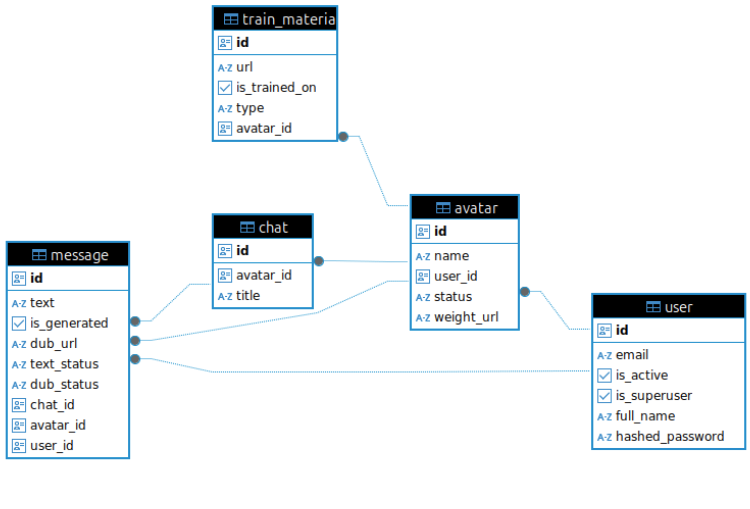
\includegraphics[width=1.0\linewidth]{images/db_structure.png}
     \caption{Структура базы данных}
     \label{fig:db_structure}
 \end{figure}



\subsection{Взаимодействие с ML-сервисом}
Взаимодействие backend с ML-сервисом осуществляется через брокер сообщений Kafka. Для работы с брокером используется библиотека aiokafka.

Чтобы обеспечить удобство поддержки и разделение ответственности, логика работы с брокером была инкапсулирована в две отдельные сущности. Критерием разделения стало направление сообщений:
\begin{itemize}
    \item KafkaMessageProducer — отвечает за формирование и отправку сообщений в ML-сервис
    \item MessageManagerConsumer — обрабатывает входящие сообщения от ML-сервиса
\end{itemize}

Такое разделение позволяет упростить масштабирование, тестирование и модификацию каждого компонента в будущем, а также не накладывает ограничений на возможность параллельной разработки.


\subsubsection{Формирование и передача запросов к ML-сервису}
KafkaMessageProducer представляет собой клиентский модуль, отвечающий за отправку заранее сформированных сообщений в Kafka. Для каждого типа сообщения реализована отдельная функция, которая использует интерфейс клиента для передачи данных в брокер.\newline
Типы сообщений:
\begin{itemize}
    \item \texttt{start\_train} — запускает обучение аватара
    \item \texttt{stop\_train} — останавливает процесс обучения;
    \item \texttt{inference\_response} — инициирует генерацию текстового ответа на сообщение пользователя;
    \item \texttt{sound\_inference} — запускает синтез озвучки для сгенерированного текста.
\end{itemize}

1. Сообщение \texttt{start\_train}
\begin{lstlisting}[style=jsonstyle, numbers=none, frame=none]
{
   "event": "train_start",
   "avatar_id": avatar_id,
   "train_materials": [
      {
         "id": material.id,
         "type": material.type,
         "url": material.url
      }
   ]
}
\end{lstlisting}
Описание полей:
\begin{itemize}
    \item \texttt{event} - тип события
    \item \texttt{avatar\_id} - уникальный идентификатор аватара
    \item \texttt{train\_materials} - список объектов для обучения:
    \begin{itemize}
        \item \texttt{id} - уникальный идентификатор материала
        \item \texttt{type} - тип материала
        \item \texttt{url} - путь в S3
    \end{itemize}
\end{itemize}

2. Сообщение \texttt{stop\_train}
\begin{lstlisting}[style=jsonstyle, numbers=none, frame=none]
{
   "event": "train_stop",
   "avatar_id": avatar_id
}
\end{lstlisting}
Описание полей:
\begin{itemize}
    \item \texttt{event} - тип события
    \item \texttt{avatar\_id} - уникальный идентификатор аватара
\end{itemize}

3. Сообщение \texttt{inference\_response}
\begin{lstlisting}[style=jsonstyle, numbers=none, frame=none]
{
   "event": "inference_response",
   "message_id": message_id,
   "text": user_message
}
\end{lstlisting}
Описание полей:
\begin{itemize}
    \item \texttt{event} - тип события
    \item \texttt{message\_id} - уникальный идентификатор сообщения пользователя
    \item \texttt{text} - текст сообщения пользователя
\end{itemize}

3. Сообщение \texttt{sound\_inference}
\begin{lstlisting}[style=jsonstyle, numbers=none, frame=none]
{
    "event": "sound_inference",
    "storage_url": storage_url,
    "base_voice_url": base_voice_url,
    "message_id": message_id,
    "text": gen_message,
}
\end{lstlisting}
Описание полей:
\begin{itemize}
    \item \texttt{event} - тип события
    \item \texttt{storage\_url} - путь в S3, где нужно будет сохранить результат
    \item \texttt{base\_voice\_url} - путь в S3, откуда брать голос для озвучки
    \item \texttt{message\_id} - уникальный идентификатор сообщения, для которого требуется озвучка
    \item \texttt{text} - текст сообщения, которое нужно озвучить
\end{itemize}

\subsubsection{Получение и обработка ответов от ML-сервиса}
Как было сказано в начале раздела - для обработки сообщений от ML-сервиса был реализован отдельный класс, MessageManagerConsumer принимает и обрабатывает все входящие сообщения. В текущей архитектуре сервис поддерживает всего два типа сообщений:
\begin{itemize}
    \item \texttt{save\_response} - сохранение сгенерированного ответа
    \item \texttt{save\_response\_dub} - сохранение сгенерированной озвучки
\end{itemize}
Учитывая небольшое количество сообщений и отсутствие планов по расширению модели сообщений в направлении от ML-сервиса к backend-сервису, а также большую схожесть в процессе обработки, было решено инкапсулировать всю логику работы внутрь единого класса. Такой подход предоставил ряд преимуществ:
\begin{itemize}
    \item Отсутствие избыточного разделения кода
    \item Единая точка отказа для данного направления
    \item Прозрачность потока данных
\end{itemize}
\begin{lstlisting}[language=Python, numbers=none, frame=none]
async with db_context() as session:
            message_id = task_data["message_id"]

            db_message = await message_repository.get_message_by_id(
                session=session,
                message_id=message_id
            )
            if db_message is None:
                logger.warning(f"Message with ID {message_id} not found.")
                return

            if event == "save_response":
                db_message.text = task_data.get(
                    "generated_text", db_message.text
                )
                db_message.text_status = "ready"

            elif event == "save_response_dub":
                db_message.text = task_data.get(
                    "generated_text", db_message.text
                )
                db_message.text_status = "ready"
                db_message.dub_url = task_data.get(
                    "dub_url", db_message.dub_url
                )
                db_message.dub_status = "ready"

            session.add(db_message)
            await session.commit()
\end{lstlisting}
1. Обработка сообщения \texttt{save\_response}\newline
В этом сообщении присутствует 3 поля:
\begin{itemize}
    \item \texttt{event} - тип события
    \item \texttt{message\_id} - уникальный идентификатор сообщения
    \item \texttt{generated\_text} - сгенерированный текст 
\end{itemize}
По \texttt{message\_id} производится поиск нужной записи в БД, после чего обновляется поле \texttt{text\_status}, которое является идентификатором готовности ответа, и \texttt{generated\_text}, которое отвечает за хранение сгенерированного ответа.\newline
2. Обработка сообщения \texttt{save\_response\_dub}\newline
В этом сообщении присутствует 4 поля:
\begin{itemize}
    \item \texttt{event} - тип события
    \item \texttt{message\_id} - уникальный идентификатор сообщения
    \item \texttt{generated\_text} - сгенерированный текст 
    \item \texttt{dub\_url} - путь в S3, где хранится озвучка 
\end{itemize}
Аналогично предыдущему пункту по \texttt{message\_id} производится поиск нужной записи в БД, после чего обновляется поле \texttt{text\_status}, \texttt{generated\_text} и \texttt{dub\_url}, а также \texttt{dub\_status}

\subsection{Взаимодействие с S3-хранилищем}
Для работы с объектным хранилищем в проекте используется MinIO — высокопроизводительная S3-совместимая платформа для хранения данных. Взаимодействие реализовано через класс-клиент, который предоставляется библиотекой. Через него можно производить базовые операции над файлами:
\begin{itemize}
    \item Загрузка
    \item Скачивание
    \item Удаление
\end{itemize}

\subsubsection{Загрузка данных пользователя}
Загрузка данных в объектное хранилище инкапсулирована в отдельную функцию: 
\begin{lstlisting}[language=Python, numbers=none, frame=none]
async def upload_to_s3(
    file: UploadFile,
    user_id: uuid.UUID,
    avatar_id: uuid.UUID,
    type: str,
    session: SessionDep
) -> str:
    file_ext = file.filename.split('.')[-1]
    file_type = detect_file_type(file_ext)
    file_id = uuid.uuid4()
    object_name = f"users/{user_id}/avatars/{
        avatar_id}/{file_type}/{file_id}.{file_ext}"

    logger.info(f"Uploading file to MinIO: {object_name}")
    logger.info(f"File type detected: {file_type}")
    logger.info(f"File type requested: {type}")
    logger.info(f"File extension: {file_ext}")

    if type == TRAINIGN_MATERIAL_TYPE.voice_syntesis and file_ext != "wav":
        logger.error(
            f"Invalid file type for voice synthesis: {
                file_type}. Expected wav."
        )
        raise HTTPException(
            status_code=400,
            detail="Invalid file type for voice synthesis. "
            "Expected audio file with wav extension for better quality."
        )

    try:
        file_data = await file.read()
        file_size = len(file_data)

        kwargs = dict(
            bucket_name=settings.MINIO_BUCKET,
            object_name=object_name,
            data=BytesIO(file_data),
            length=file_size,
            content_type=file.content_type,
        )
        await run_in_threadpool(minio_client.put_object, **kwargs)
    except S3Error as exc:
        raise RuntimeError(f"Failed to upload to MinIO: {exc}")

    if type == TRAINIGN_MATERIAL_TYPE.voice_syntesis and file_ext == "wav":
        await avatar_repository.update_avatar_voice_url(
            session=session,
            avatar_id=avatar_id,
            voice_url=f"{
                settings.MINIO_URL}/{settings.MINIO_BUCKET}/{object_name}"
        )

    return f"{settings.MINIO_URL}/{settings.MINIO_BUCKET}/{object_name}"
\end{lstlisting}
Стоит обратить внимание, что все файлы для обучения сохраняются по этому пути:\newline
\texttt{users/\{user\_id\}/avatars/\{avatar\_id\}/\{file\_type\}/\{file\_id\}.\{file\_ext\}}\newline
Преимущества такой организации файлов:
\begin{itemize}
    \item Консистентность между хранилищем и API - пути в S3 зеркалируют структуру маршрутов
    \item Единая логика доступа - упрощает построение ментальной модели, что помогает увеличить скорость разработки
    \item Прозрачность взаимодействия - иерархия путей сохраняет отношения между сущностями
    \item Масштабируемость - позволяет легко добавлять новые уровни вложенности
\end{itemize}


\section{Сервис генерации звука}

Сервис реализован как отдельное приложение, функционирующее в режиме
фонового процесса и обрабатывающее сообщения из системы обмена сообщениями
Kafka. В зависимости от параметров задачи он способен использовать как
основную нейросетевую модель синтеза речи (xtts\_v2), так и альтернативную — LLASA.
Хранение аудиофайлов реализовано через объектное хранилище MinIO.

\subsection{Обработка событий брокера сообщений и инициализация очереди генерации}
После старта приложение инициализирует Kafka-консюмера и подписывается
на два ключевых топика: \textbf{sound\_inference} (обработка задач озвучки)
и \textbf{health\_check} (мониторинг работоспособности). Эта инициализация
происходит в точке входа:

\begin{lstlisting}[language=Python, numbers=none, frame=none]
consumer = KafkaMessageConsumer(
    bootstrap_servers=settings.KAFKA_BROKER_URL,
    topics=[
        settings.KAFKA_HEALTH_CHECK_TOPIC,
        settings.KAFKA_TOPIC_SOUND_INFERENCE,
    ],
    group_id=settings.KAFKA_GROUP_ID
)
consumer.run()
\end{lstlisting}

Консюмер постоянно опрашивает брокер Kafka, проверяя наличие новых сообщений,
и при получении валидной задачи вызывает функцию обработки:

\begin{lstlisting}[language=Python, numbers=none, frame=none]
def execute_task_pipeline(task_data):
    curr_event = task_data["event"]

    if curr_event == "sound_inference":
        process_inference_task(task_data)
\end{lstlisting}

\subsection{Этапы синтеза речи}
При поступлении задачи с типом \textbf{sound\_inference} запускается пайплайн,
использующий Coqui TTS (модель \textbf{xtts\_v2}). Модель загружается при первом
обращении и используется для синтеза речи на основе текста и выбранного голосового профиля.

В зависимости от параметров задачи, может быть использован как кастомный голос,
загружаемый из MinIO, так и предустановленный:

\begin{lstlisting}[language=Python, numbers=none, frame=none]
if base_voice:
    tts.tts_to_file(
        text=text,
        language='ru',
        speaker_wav=temp,
        pipe_out=wrapper
    )
else:
    tts.tts_to_file(
        text=text,
        language='ru',
        speaker='Craig Gutsy',
        pipe_out=wrapper
    )
\end{lstlisting}

Полученный аудиофайл сохраняется в MinIO. Для этого используется обёртка
над \texttt{BytesIO} и функция загрузки:

\begin{lstlisting}[language=Python, numbers=none, frame=none]
def save_dub_to_s3(dub_url: str, buffer: io.BytesIO) -> str:
    buffer.seek(0)
    minio_client.put_object(
        bucket_name=settings.MINIO_BUCKET,
        object_name=dub_url,
        data=buffer,
        length=buffer.getbuffer().nbytes,
        content_type='audio/wav'
    )
    return dub_url
\end{lstlisting}

Перед генерацией, если используется кастомный голос, он временно скачивается
в локальное хранилище:

\begin{lstlisting}[language=Python, numbers=none, frame=none]
def download_minio_file_to_local(object_name: str, suffix: str = ".wav") -> str:
    response = minio_client.get_object(
        bucket_name=settings.MINIO_BUCKET,
        object_name=object_name,
    )
    with tempfile.NamedTemporaryFile(delete=False, suffix=suffix) as temp_file:
        temp_file.write(response.read())
    return temp_file.name
\end{lstlisting}

По завершении — временный файл удаляется:

\begin{lstlisting}[language=Python, numbers=none, frame=none]
def delete_local_file(file_path: str) -> None:
    if os.path.exists(file_path):
        os.remove(file_path)
\end{lstlisting}

После успешного завершения обработки, результат отправляется обратно в Kafka:

\begin{lstlisting}[language=Python, numbers=none, frame=none]
def send_update_message_state(producer, message_id, generated_text, dub_url):
    payload = {
        "event": "save_response_dub",
        "message_id": str(message_id),
        "dub_url": dub_url,
        "generated_text": generated_text,
    }
    producer.send(topic=settings.KAFKA_TOPIC_SAVE_RESPONSE_DUB, data=payload)
\end{lstlisting}


Альтернативный режим работы используется, если в задаче явно указан режим
\texttt{llasa}. В этом случае применяется модель LLASA в связке с декодером Codec2.
Генерация выполняется в несколько этапов:

\begin{itemize}
\item Формирование промпта с использованием специальных токенов;
\item Токенизация текста с помощью LLASA;
\item Генерация модели и извлечение токенов;
\item Декодирование в аудиосигнал с помощью Codec2.
\end{itemize}

\begin{lstlisting}[language=Python, numbers=none, frame=none]
chat = [
    {
        "role": "user",
        "content": "Convert the text to speech: <|TEXT_UNDERSTANDING_START|>...<|TEXT_UNDERSTANDING_END|>"
    },
    {
        "role": "assistant",
        "content": "<|SPEECH_GENERATION_START|>"
    }
]
in_ids = tokenizer.apply_chat_template(chat, tokenize=True, return_tensors='pt')
outputs = model.generate(...)
\end{lstlisting}

\subsection{Формат обратной связи через брокер сообщений}
После завершения генерации, итоговое сообщение, отправляемое обратно в Kafka,
имеет унифицированный JSON-формат:

\begin{lstlisting}[style=jsonstyle, numbers=none, frame=none]
{
    "event": "save_response_dub",
    "message_id": "e4aa6ae7-d6d6-4b1a-88fc-6d79a50a645f",
    "dub_url": "avatars/.../dubs/1ddf...wav",
    "generated_text": "some text"
}
\end{lstlisting}

Поля сообщения включают:
\begin{itemize}
\item \textbf{event} — тип события (\texttt{save\_response\_dub});
\item \textbf{message\_id} — уникальный идентификатор запроса;
\item \textbf{dub\_url} — путь к аудиофайлу в хранилище;
\item \textbf{generated\_text} — сгенерированный текст ответа.
\end{itemize}


Сервис генерации озвучки представляет собой устойчивое и расширяемое звено
архитектуры Bishop. Он позволяет не только получить текстовый ответ, но и
воспроизвести его голосом, делая взаимодействие с системой ближе к
естественному. Гибкость реализации позволяет легко адаптировать сервис под
новые задачи и модели.


\section{Сервис генерации текста}
Сервис реализует два основных пайплайна: пайплайн генерации текста и пайплайн обучения модели. Оба пайплайна построены из независимых, переиспользуемых компонентов, в соответствии с принципами чистой архитектуры, что позволяет гибко адаптировать процессы под изменение базовой модели и требований к системе. Архитектура сервиса во многом схожа с архитектурой сервиса генерации звука: взаимодействие между компонентами осуществляется посредством сообщений, поступающих через Kafka. Сервис ожидает команды на запуск соответствующего пайплайна, а после завершения работы формирует и отправляет результат обратно через Kafka.

\subsection{Пайплайн обучения модели}
Обучение модели является ресурсозатратной и длительной по времени операцией, поэтому запуск реализован как отдельный процесс. Благодаря этому он остается доступным и может сообщать другим компонентам системы о текущем состоянии обучения, не блокируя основной поток.

Для контроля состояния процесса и исключения повторного запуска одновременно нескольких экземпляров пайплайна, используется механизм хранения информации о процессе в Redis. Это реализовано через класс RedisManager на основе библиотеки redis, который предоставляет методы для записи, чтения и удаления информации о текущем обучении. Таким образом, если процесс уже запущен, повторный запуск будет отклонен, потому что предполагается, что все ресурсы системы в это время заняты.

Для запуска и контроля отдельного процесса используются функции на основе библиотеки multiprocessing, выделенные в отдельный инфраструктурный менеджер, реализующие запуск задачи в отдельном процессе, проверка есть ли запущенный процесс и возможность принудительного завершения процесса:
\begin{lstlisting}[language=Python, numbers=none, frame=none]
def run_task_in_process(func, *args):
    if is_process_running():
        logger.warning("A process is already running. Rejecting new request.")
        return

    logger.info("Launching task in a separate process")
    p = Process(target=func, args=args)
    p.start()

    redis_manager.set_running_process_id(p.pid)
    logger.info(f"Started task with PID {p.pid}")

def is_process_running() -> bool:
    process_id = redis_manager.get_running_process_id()
    if process_id:
        logger.info(f"Process with PID {process_id} is already running.")
        return True
    return False

def terminate_process(pid: int) -> bool:
    try:
        os.kill(pid, signal.SIGTERM)
        logger.info(
            f"Successfully sent termination signal to process with PID {pid}")
        return True
    except ProcessLookupError:
        logger.warning(f"Process with PID {pid} not found.")
        return False
    except Exception as e:
        logger.error(f"Error while trying to terminate process {pid}: {e}")
        return False
\end{lstlisting}

\subsubsection{Этап подготовки данных}
После запуска отдельного процесса обучения первым этапом является обработка данных, включающая в себя три этапа:
\begin{itemize}
\item Загрузка всех файлов из S3-хранилища:
\begin{lstlisting}[language=Python, numbers=none, frame=none]
def download_data(
        s3_urls: List[Path],
        output_dir: Path = Path(settings.RAW_DATA_DIR),
) -> List[Path]:
    logger.info("Processing dataset...")
    local_files = []

    for s3_url in tqdm(s3_urls, desc="Downloading files"):
        try:
            local_path = s3_storage.download_file(s3_url)
            local_files.append(local_path)
        except Exception as e:
            logger.error(f"Error downloading {s3_url}: {e}")

    logger.info(f"Processing dataset complete. Files saved to {output_dir}")
    return local_files
\end{lstlisting}
\item Извлечение аудио и транскрипция.  Для этого используется класс Transcribator, основанный на библиотеке moviepy для извлечения аудио из видео и модели Whisper от OpenAI для транскрипции звуковых дорожек в текст:
\begin{lstlisting}[language=Python, numbers=none, frame=none]
class Transcribator:
    def __init__(self, model_type: str = "base"):
        self.model_type = model_type
        self.model = whisper.load_model(self.model_type)

    def transcribe_audio(
            self,
            audio_path: Path,
            output_dir: Path = Path(settings.INTERIM_DATA_DIR),
    ) -> Path:
        output_dir.mkdir(parents=True, exist_ok=True)
        result = self.model.transcribe(str(audio_path))
        output_path = output_dir / (audio_path.stem + ".txt")
        with output_path.open('w', encoding='utf-8') as f:
            f.write(result['text'])
        return str(output_path)

    def transcribe_video(
            self,
            video_path: Path,
            output_dir: Path = Path(settings.INTERIM_DATA_DIR),
    ) -> Path:
        output_dir.mkdir(parents=True, exist_ok=True)
        temp_audio = output_dir / "temp_audio.wav"
        try:
            video = VideoFileClip(str(video_path))
            video.audio.write_audiofile(str(temp_audio), codec='pcm_s16le', logger=None)
            video.close()
            result = self.model.transcribe(str(temp_audio))
            output_path = output_dir / (video_path.stem + ".txt")
            with output_path.open('w', encoding='utf-8') as f:
                f.write(result['text'])
            return str(output_path)
        finally:
            if temp_audio.exists():
                temp_audio.unlink()
\end{lstlisting}
\item Формирование финального датасета. Происходит очистка текста от символов разметки и разделение длинных строк на разные:
\begin{lstlisting}[language=Python, numbers=none, frame=none]
def _clean_text(text: str) -> str:
    text = re.sub(r"<[^>]+>", "", text)
    text = normalize("NFKC", text)
    text = re.sub(r"\s+", " ", text)
    return text.strip()


def _split_into_chunks(text: str, max_len: int = 1000, min_len: int = 50) -> list[str]:
    text = text.replace("\r\n", "\n").replace("\r", "\n")

    rough_chunks = re.split(r"\n{2,}|\.\s", text)
    refined_chunks = []

    for chunk in rough_chunks:
        chunk = chunk.strip()
        if len(chunk) < min_len:
            continue

        if not re.search(r"[.,!?…]", chunk):
            i = 0
            while i < len(chunk):
                max_rand_len = min(max_len, len(chunk) - i)
                if max_rand_len < min_len:
                    break
                rand_len = random.randint(min_len, min(max_len, len(chunk) - i))
                part = chunk[i:i + rand_len].strip()
                if len(part) >= min_len:
                    refined_chunks.append(part)
                i += rand_len
            continue

        while len(chunk) > max_len:
            split_idx = chunk.rfind(" ", 0, max_len)
            if split_idx == -1:
                split_idx = max_len
            part = chunk[:split_idx].strip()
            if len(part) >= min_len:
                refined_chunks.append(part)
            chunk = chunk[split_idx:].strip()
        if len(chunk) >= min_len:
            refined_chunks.append(chunk)

    return refined_chunks


def build_dataset(
    input_dir: Path = Path(settings.INTERIM_DATA_DIR),
    output_file: Path = Path(settings.PROCESSED_DATA_DIR) / "dataset.txt",
) -> Path:
    output_file.parent.mkdir(parents=True, exist_ok=True)
    text_files = list(input_dir.glob("*.txt"))

    all_chunks = []

    for file in text_files:
        raw_text = file.read_text(encoding="utf-8")
        if not raw_text.strip():
            continue
        cleaned = _clean_text(raw_text)
        chunks = _split_into_chunks(cleaned)
        all_chunks.extend(chunks)

    unique_chunks = list(dict.fromkeys(all_chunks))

    with output_file.open("w", encoding="utf-8") as f_out:
        for chunk in unique_chunks:
            f_out.write(chunk + "\n")

    logger.info(f"Cleaned dataset with {len(unique_chunks)} samples saved at {output_file}")
    return output_file
\end{lstlisting}
\end{itemize}

\subsubsection{Этап запуска обучения}
Следующим этапом после формирования датасета является обучение модели, реализованного на библиотеках datasets и transformers. В зависимости от конфигурации, обучение может происходить локально либо на платформе Kaggle, где процесс контролируется и отслеживается через API. Управление этим шагом реализовано с помощью класса KaggleManager, который инкапсулирует всю логику взаимодействия с Kaggle API, включая аутентификацию, загрузку датасета, запуск Python-скрипта, отслеживание его выполнения и скачивание результатов:
\begin{lstlisting}[language=Python, numbers=none, frame=none]
class KaggleManager:

    def __init__(self) -> None:
        self._api = KaggleApi()

    def authenticate(self) -> None:
        try:
            self._api.authenticate()
        except Exception as e:
            raise KaggleAuthenticationError("Failed to authenticate with Kaggle API") from e

    def upload_dataset(self, dataset_dir: Path) -> None:
    
        dataset_config_path = self._generate_dataset_config(dataset_dir)

        try:
            self._api.dataset_create_version(
                folder=dataset_dir,
                version_notes="A universal version of the dataset for launching training",
            )
            logger.info(f"Dataset uploaded successfully from {dataset_dir}."
                        f"Waiting 7 seconds for Kaggle to update the data.")
            time.sleep(7)

            dataset_config_path.unlink(missing_ok=True)
            logger.info("Dataset metadata file deleted.")
        except Exception as e:
            raise KaggleManagerError(f"Failed to create a new version of the dataset from {dataset_dir}.") from e

    def run_script(self, py_script_path: Path) -> str:
        self.__generate_py_script_config(py_script_path)

        try:
            logger.info(f"Uploading python script {py_script_path} to Kaggle...")
            response = self._api.kernels_push(
                folder=py_script_path.parent,
                timeout=settings.KAGGLE_KERNEL_RUN_TIMEOUT,
            )
            logger.info(f"Python script {py_script_path} uploaded successfully.")

            py_script_path.unlink(missing_ok=True)
            logger.info(f"Kernel metadata deleted.")

            kernel_ref = f"{settings.KAGGLE_AUTH_NAME}/{settings.KAGGLE_KERNEL_TITLE}"
            return kernel_ref
        except Exception as e:
            raise KaggleManagerError(f"Failed to upload python script {py_script_path} to Kaggle.") from e

    def track_execution(self, kernel_ref: str) -> None:
        while True:
            status_response = self._api.kernels_status(kernel_ref)
            status = status_response.status.name

            if status == "COMPLETE":
                logger.info(f"Kernel '{kernel_ref}' completed successfully.")
                return
            elif status in (
                    "ERROR",
                    "CANCEL_REQUESTED",
                    "CANCEL_ACKNOWLEDGED",
            ):
                error_msg = f"Kernel '{kernel_ref}' failed with status: {status}"
                if failure_message := status_response.failure_message:
                    error_msg += f" | Message: {failure_message}"
                raise RuntimeError(error_msg)
            elif status == "QUEUED":
                logger.info(f"Kernel '{kernel_ref}' is in queue...")
                time.sleep(5)
            elif status in (
                    "RUNNING",
                    "NEW_SCRIPT"
            ):
                logger.info(f"Kernel '{kernel_ref}' is in progress...")
                time.sleep(3)

    def download_output(self, kernel_ref: str, output_dir: Path) -> List[Path]:
        if not output_dir.exists():
            output_dir.mkdir(parents=True, exist_ok=True)

        if not output_dir.is_dir():
            raise ValueError("Provided path must be a directory.")

        try:
            logger.info(f"Downloading output of kernel '{kernel_ref}' to '{output_dir}'...")
            outfiles, token = self._api.kernels_output(
                kernel=kernel_ref,
                path=output_dir,
                force=True
            )
            logger.info(f"Downloading output of kernel '{kernel_ref}' to '{output_dir}' completed successfully.")
        except Exception as e:
            raise RuntimeError(f"Failed to download output for kernel '{kernel_ref}'") from e

        if not outfiles:
            logger.warning(f"No output files found for kernel '{kernel_ref}'")
        else:
            logger.info(f"Downloaded {len(outfiles)} files from kernel '{kernel_ref}'")

        return [Path(f) for f in outfiles]

    def __generate_py_script_config(self, py_script_path: Path) -> None:
        if not py_script_path.is_file():
            raise ValueError(f"Provided python script path {py_script_path} is not a valid file.")

        kernel_metadata_file = py_script_path.parent / "kernel-metadata.json"

        dataset_ref = f"{settings.KAGGLE_AUTH_NAME}/{settings.KAGGLE_DATASET_TITLE}"

        kernel_metadata = {
            "id": f"{settings.KAGGLE_AUTH_NAME}/{settings.KAGGLE_KERNEL_TITLE}",
            "title": settings.KAGGLE_KERNEL_TITLE.replace("-", " ").capitalize(),
            "code_file": py_script_path.name,
            "language": "python",
            "kernel_type": "script",
            "is_private": True,
            "enable_gpu": True,
            "enable_tpu": False,
            "enable_internet": True,
            "dataset_sources": [dataset_ref],
            "competition_sources": [],
            "kernel_sources": [],
            "model_sources": [],
        }

        with open(kernel_metadata_file, 'w') as f:
            json.dump(kernel_metadata, f, indent=4)

        logger.info(f"Kernel metadata created at {py_script_path}")

    def _generate_dataset_config(self, dataset_dir: Path) -> Path:
        if not dataset_dir.is_dir():
            raise ValueError(f"Provided dataset folder path {dataset_dir} is not a valid directory.")

        dataset_metadata_file = dataset_dir / "dataset-metadata.json"

        dataset_metadata = {
            "id": f"{settings.KAGGLE_AUTH_NAME}/{settings.KAGGLE_DATASET_TITLE}",
            "title": settings.KAGGLE_DATASET_TITLE.replace("-", " ").capitalize(),
            "licenses": [{"name": "CC0-1.0"}],
            "is_public": False,
        }

        with open(dataset_metadata_file, 'w') as f:
            json.dump(dataset_metadata, f, indent=4)

        logger.info(f"Dataset metadata created at {dataset_metadata_file}")

        return dataset_metadata_file
\end{lstlisting}

\subsubsection{Этап сохранения результатов}
Завершающим этапом пайплайна обучения является сохранение результатов в S3 и отправка сообщения об окончании в Kafka. Обученная модель передаётся с помощью метода upload\_file() класса S3StorageWithCache. Этот класс реализует работу с объектным хранилищем на базе библиотеки MinIO:
\begin{lstlisting}[language=Python, numbers=none, frame=none]
class S3StorageWithCache:
    def __init__(
        self,
        cache_dir: Path,
    ):
        self.client = minio_client
        self.bucket_name = settings.MINIO_BUCKET
        self.cache_dir = cache_dir
        self.cache_dir.mkdir(parents=True, exist_ok=True)

     def upload_file(self, local_path: Path, object_key: str):
        self.client.fput_object(
            bucket_name=self.bucket_name,
            object_name=object_key,
            file_path=str(local_path),
        )

        logger.info(f"Uploaded file {local_path}, with object_key {object_key}")
\end{lstlisting}